\chapter{Ejercicio Sigue Personas simulado en Robotics Academy}
\label{cap:capitulo5}

En este capítulo se presenta la elaboración del ejercicio \textbf{Follow Person} para Robotics Academy empezando desde el desarrollo interno de la infraestructura del ejercicio hasta una solución óptima de referencia que realice la tarea de seguir a una persona.



% -- SECCION ENTORNO GAZEBO
% ---------------------------
\section{Entorno simulado de un hospital}
\label{sec:hospital_gazebo}

La primera tarea fue integrar un \textbf{escenario} para Gazebo en el cual el robot Turtlebot 2 tendría que enfrentarse. El escenario candidato que elegimos fue un \textbf{Hospital} debido a las siguientes ventajas:

\begin{enumerate}
	\item El robot se enfrenta a un \textbf{entorno complejo} (paredes, obstáculos, varias personas).
	\item La tarea Sigue Personas tiene lugar en un entorno en el cuál tiene sentido verlo en el mundo real. Los Robots en el ámbito de la \textbf{salud} están en continua integración y más desde el año 2020.
\end{enumerate}

De modo que incorporamos el siguiente escenario de Gazebo que proporciona AWS (Amazon Web Service) en uno de sus repositorios de Github \footnote{\textbf{aws hospital}: \url{https://github.com/aws-robotics/aws-robomaker-hospital-world}}:\\

\begin{figure} [H]
  \begin{center}
    \includegraphics[width=10cm]{imagenes/hospital_world.png}
  \end{center}
  \caption[Hospital de AWS en Gazebo]{Hospital de AWS en Gazebo}
  \label{fig:hospital_gazebo}
\end{figure}\

El repositorio proporcionaba varios ficheros \textbf{.world} con distintas versiones del Hospital: solo planta baja, una planta y dos plantas. Elegimos por comodidad la primera.\\

El siguiente paso era integrar una persona que pudiera desplazarse por el entorno.\\



% -- SECCION TELEOPERADOR
% -------------------------
\section{Teleoperador}
\label{sec:teleoperador}

La meta final es que el usuario que use la plantilla web pueda controlar \textbf{manualmente} una persona del Hospital para que el robot pueda seguirla. Para ello teníamos que desarrollar un \textbf{teleoperador}.\\

El primer punto de partida era integrar una persona en el nuevo entorno simulado, por lo que accedimos a este repositorio \footnote{\url{https://github.com/osrf/gazebo_models}} que incorpora una librería de modelos para Gazebo e insertamos en el repositorio de Robotics Academy de terceros \textbf{Custom Robots} el modelo \textbf{\textit{person standing}}\\

\begin{figure} [H]
  \begin{center}
    \includegraphics[width=10cm]{imagenes/person_model.png}
  \end{center}
  \caption[Persona simulada en Gazebo]{Persona simulada en Gazebo}
  \label{fig:persona_gazebo}
\end{figure}\

Ahora bien, el modelo es \textbf{estático}, carece de capacidad de desplazamiento, por lo que fue necesario desarrollar un \textbf{plugin} para Gazebo que permitiera controlarlo o que pudiera desplazarse a través de una ruta que eligiera el programador. De modo que en el mismo paquete donde teníamos los ficheros de lanzamiento del hospital diseñamos el plugin (escrito en C++) que denominamos \textbf{libpersonplugin.so} para incorporarlo en el fichero \textbf{.sdf} (similar a URDF) de la persona. En este enlace podréis ver el \textbf{código fuente}\footnote{\textbf{person plugin}: \url{https://github.com/JdeRobot/CustomRobots/blob/foxy-devel/amazon_hospital/hospital_world/src/person.cpp}}. Como punto de partida, tomé como referencia un plugin de una persona simulada que hizó \textit{Pedro Arias} en su TFM\footnote{\textbf{TFM Pedro Arias}: \url{https://github.com/RoboticsLabURJC/2021-tfm-pedro-arias}}\\

El plugin requiere \textbf{2 funcionalidades}:
\begin{enumerate}
	\item \textbf{Comunicación remota} para el control manual. La intención es que el usuario se comunique con el modelo simulado, por lo tanto se ha diseñado un \textbf{socket} de comunicaciones para dicha tarea.
	\item \textbf{Establecimiento de una ruta} por defecto y capacidad de incorporar nuevas rutas. Esta última funcionalidad no es necesaria para el ejercicio, además de que puede suponer cierta molestia al usuario, pero no se descarta su utilidad para un futuro. Básicamente, dado un vector de tuplas de tipo $<$float, float, int$>$ donde los 2 primeros elementos indican la posición X e Y y el último parámetro apuntando al siguiente punto de paso, podemos implementar una ruta en un bucle infinito (el último punto de paso tiene que apuntar al primero).
\end{enumerate}\




% -- SUBSECCION COMUNICACION REMOTA
% ----------------------------------
\subsection{Comunicación remota}
\label{subsec:comunicacion_remota}

En el propio fichero \textbf{person.cpp} se crearon \textbf{2 hilos} (threads): uno actuaría como \textbf{servidor} de un socket de comunicaciones que usaría el protocolo de transporte \textbf{UDP} (No esta orientado a la conexión y es más rápido) y otro hilo se encargaría de actualizar la posición del modelo. Dentro del socket se implementó un \textbf{protocolo} de comunicación que entendierá el servidor, el cual se comportara únicamente como receptor de los mensajes del cliente. Los \textbf{mensajes} (de 3 caracteres) que puede recibir son:\\

\begin{itemize}
	\item \textbf{``UVF"} (User Velocity Forward). El modelo se mueve hacia delante.
	\item \textbf{``UVB"} (User Velocity Backward). El modelo se mueva hacia atrás.
	\item \textbf{``UAR"} (User Angular Right). El modelo gira hacia la derecha.
	\item \textbf{``UAL"} (User Angular Left). El modelo gira hacia la izquiera.
	\item \textbf{``US-"} (User Stop). El modelo se detiene.
	\item \textbf{``A--"} (Autonomous). El modelo pasa a modo autónomo. Sigue la ruta establecida (actualmente desactivada).
\end{itemize}\

Pero ¿dónde entra en juego el cliente? El fichero \textbf{exercise.py} incorpora un socket de comunicación UDP que se conecta al servidor del plugin a través del puerto 36677. Además, el \textbf{exercise.py} es el \textbf{servidor} de un WebSocket en comunicación con la plantilla web. Cuando el usuario haga click en el botón ``Teleoperate", el fichero de \textbf{eventos} de Javascript enviará a través de un Websocket (usa el puerto 1905) las teclas pulsadas para que el exercise.py se lo retransmita al plugin. Al iguál que en la comunicación \textbf{plugin-exercise.py}, implementé un protocolo de comunicación para \textbf{exercise.py-exercise.html}. Los \textbf{mensajes} que puede recibir son:\\

\begin{itemize}
	\item \textbf{``\#teleop\_true"}. Activa la \textbf{teleoperación}. A partir de ese momento, el usuario puede pulsar los botones ``awsdx". Envía un mensaje \textbf{``US-"} al plugin.
	\item \textbf{``\#teleop\_false"}. Desactiva la teleoperación. Pasa a modo autónomo (si estuviera activado). Envía una mensaje \textbf{``A--"} al plugin.
	\item \textbf{``\#key\_a"}. Envía un mensaje \textbf{``UAR"} al plugin.
	\item \textbf{``\#key\_d"}. Envía un mensaje \textbf{``UAL"} al plugin.
	\item \textbf{``\#key\_w"}. Envía un mensaje \textbf{``UVF"} al plugin.
	\item \textbf{``\#key\_s"}. Envía un mensaje \textbf{``UVB"} al plugin.
	\item \textbf{``\#key\_x"}. Envía un mensaje \textbf{``US-"} al plugin.
\end{itemize}\

A continuación podemos ver un esquema que resuma la comunicación existente entre el exercise.html (incorpora el fichero ws\_code.js que es el manejador de eventos del menú superior de la plantilla web) con el plugin:\\

\begin{figure} [H]
  \begin{center}
    \includegraphics[width=15cm]{imagenes/comunicacion-teleoperador.png}
  \end{center}
  \caption[Comunicación del teleoperador]{Comunicación del teleoperador}
  \label{fig:comunicacion_teleoperador}
\end{figure}\

\cleardoublepage


% -- SECCION RNA
% ----------------
\section{Elección la RNA para detección de Objetos}
\label{sec:eleccion_rna}

La elección de una RNA que pueda detectar objetos se basó en este \textbf{criterio}: tiene que procesar óptimamente en una CPU y o en un contenedor Docker sin aceleración gráfica para permitir al usuario la ópción de programar cómodamente y poder disfrutar igualmente de la experiencia. Para ello, hicimos un previo estudio de los FPS cuando se usa estos 2 modelos de RNA en una aplicación de Visión Artificial: Darknet ROS y SSD Inceptión V2 (ambos introducidos en el capítulo 1).\\

Primero probamos un paquete \textit{fork}\footnote{\textbf{Darknet ROS}: \url{https://github.com/Ar-Ray-code/darknet_ros/tree/foxy/darknet_ros/}} del repositorio oficial de \textbf{Darknet ROS} para ROS 2 Foxy que incluía 1 fichero de lanzamiento \textbf{yolov4-tiny.launch.py} que ejecutaba una RNA profunda con menos capas que la original, provocando un aumento de rendimiento pero menor precisión. La ventaja de usar Darknet ROS es que indicas en un fichero de configuración el topic sobre el que se publica las imágenes de OpenCv \footnote{para la cámara IntelRealsense R200 usamos este comando para publicar la imagen sobre un topic: \textbf{ros2 run v4l2\_camera v4l2\_camera\_node --ros-args -p video\_device:="/dev/video4"}} y automáticamente la Red Neuronal procesa la imagen y publica los resultados en 3 topics: \textbf{/darknet\_ros/bounding\_boxes}, \textbf{/darknet\_ros/found\_object} y \textbf{/darknet\_ros/detection\_image}.\\

Mientras ejecutábamos Darknet ROS lanzamos este comando para medir los FPS y volcar los datos en un fichero:\\

\begin{lstlisting}
ros2 topic hz /darknet_ros/detection_image > darknet_ros_hz
\end{lstlisting}\

Después probamos la velocidad de procesamiento de la red Inception de SSD (cuyos ficheros de configuración los obtuvimos de este repositorio\footnote{\textbf{ficheros SSD}: \url{https://github.com/iitzco/OpenCV-dnn-samples/tree/master/tensorflow}}, ejecutando un programa python [\ref{cod:medicion_fps}] y mostrando los bounding boxes en pantalla (en la sección \ref{sec:sigue_personas_simulado} explicaremos cómo dibujar los Bounding Boxes). Al igual que hicimos con Darknet ROS volcamos los resultados en otro fichero.\\

\begin{code}[H]
\begin{lstlisting}
cap = cv2.VideoCapture(4)
net = NeuralNetwork()

start_time = time.time()
rate = 1
counter = 0

while True:
	ret, image = cap.read()
	
	if ret:
		detections = net.detect(image)
		
		# Process detection ...

		counter += 1
		if (time.time() - start_time) > rate:
			print("FPS: ", counter / (time.time() - start_time))
			counter = 0
			start_time = time.time()

cap.release()
\end{lstlisting}
\caption{Medición de FPS con SSD Inception}
\label{cod:medicion_fps}
\end{code}\

Una vez realizadas las 2 mediciones comprobamos los resultados mediante una gráfica de python (usando el módulo \textbf{matplotlib}). El resultado fue el siguiente:\\

\begin{figure} [H]
  \begin{center}
    \includegraphics[width=10cm]{imagenes/comparativa-fps-models.png}
  \end{center}
  \caption[Comparativa FPS entre Darknet ROS y SSD Inception]{Comparativa FPS entre Darknet ROS y SSD Inception}
  \label{fig:comparativa_fps_models}
\end{figure}\

Como vemos en la figura, Darknet ROS no funciona de manera óptima para portátiles sin GPU (media de 2.5 fps). En cambio, SSD Inception nos sorprende a priori con una velocidad de unos 25 fotogramas por segundo de media. Por tanto la elección de SSD se ve clara, sin embargo, estos resultados no serán los esperados cuando el usuario lance un contenedor Docker. Recordemos que el contenedor tendrá que lanzar ROS, un escenario de Gazebo y varios módulos de Python de manera concurrente (incluido VNC para \textit{visualización remota}), pero con SSD habremos conseguido proporcionar un ejercicio de Deep Learning con mayor nivel de procesamiento.\\




% -- SECCION HAL
% ----------------
\section{Desarrollo de la Capa de Abstracción Hardware (HAL)}
\label{sec:turtlebot2_hal_simulado}

En esta sección explicaremos el desarrollo de la Capa de Abstracción Hardware (HAL) que incluímos en este ejercicio, además de algunos nuevos cambios para su adaptación a ROS2.\\

Todos los ejercicios de Robotics Academy comparten una estructura muy similar. Tienen un fichero llamado \textbf{exercise.py} que se comunica tanto con el \textbf{navegador} como con los demás ficheros de su directorio. Partiendo de dicha ruta relativa, hay un directorio denominado \textbf{interfaces} donde encontramos ficheros python que actuan a modo de plantilla para comunicarse con nodos de ROS dedicados. En todos hubo que hacer algunas modificaciones debido al cambio de ROS 1 a ROS 2 (modo de creación de los nodos, publicadores y suscriptores). Como ficheros \textit{interfaces} tenemos la cámara, el láser, los motores, la odometría, y la detección mediante SSD Inception entre otros.\\

La gran novedad se encuentra en el fichero \textbf{ssd\_detection.py} (nueva incorporación). En él definimos la clase \textbf{BoundingBox} y la clase \textbf{NeuralNetwork}:\\

La clase \textbf{BoundingBox} tiene los siguientes atributos:
\begin{itemize}
	\item \textbf{id}: Es un entero que identifica un tipo de objeto.
	\item \textbf{class\_id}: Es una cadena de texto que identifica un tipo de objeto. Con el atributo \textbf{id} forman una pareja (clave - valor) que se puede observar en un fichero que importamos llamado \textbf{coco\_labels.py} donde se registran todos los tipos de objetos que puede detectar la red neuronal:\\
\begin{lstlisting}
LABEL_MAP = {
    0: "unlabeled",
    1: "person",
    2: "bicycle",
    3: "car",
    4: "motorcycle",
    5: "airplane",
    6: "bus",
    7: "train",
    8: "truck",
...
}
\end{lstlisting}\
	\item \textbf{score}: Es un número en coma flotante que va de 0 a 1 que indica la \textbf{probabilidad} de que el objeto detectado clasificado por la red neuronal concida con el objeto real. Su elección es causa de una selección como el objeto con mayor porcentaje de la lista \textbf{LABEL\_MAP}
	\item \textbf{xmin} e \textbf{ymin}: Indican las coordenadas (x, y) del extremo superior izquierdo del Bounding Box.
	\item \textbf{xmax} e \textbf{ymax}: Indican las coordenadas (x, y) del extremo inferior derecho del Bounding Box.
\end{itemize}\

En la clase \textbf{NeuralNetwork}, encapsulamos la importación de los ficheros que definen la red neuronal Inception: \textbf{ssd\_inception\_v2\_coco.pb} y \textbf{ssd\_inception\_v2\_coco.pbtxt}. La creación de la red neuronal se usará con OpenCv usando la función \textbf{cv2.dnn.readNetFromTensorFlow(model, config)} al que se le pasa como argumentos la ruta a los 2 ficheros citados anteriormente. Creamos un método llamado \textbf{detect(self, img)} que se encarga de llamar internamente al modelo para realizar una detección sobre una imagen.\\

Una vez creado los ficheros \textbf{interfaces} crearemos la API de HAL en el fichero \textbf{hal.py}. Nuestro módulo (que usará el usuario) tendrá las siguientes funciones:\\
\begin{itemize}
	\item \textbf{setV(velocity)}. Nos permite usar velocidades lineales. Usa la interfaz \textbf{motors} que publica sobre el topic \textbf{/cmd\_vel}
	\item \textbf{setW(velocity)}. Nos permite usar velocidades angulares (radianes). Usa también la interfaz \textbf{motors} para publicar sobre el mismo topic.
	\item \textbf{getLaserData()}. Devuelve una lista 180 lecturas del láser (para facilitar la programación al usuario y ocultar distintas calibraciones) mediante de un tipo de datos llamado \textbf{LaserData} usando la interfaz \textbf{laser} que se suscribe al topic \textbf{/scan}. El láser RPLIDAR 360 del fichero de configuración URDF está colocado de tal manera que el ángulo 0 apunta hacia delante del robot y en sentido anti-horario, por lo tanto fue necesario retornar 180 valores del láser en el orden que mostramos en la figura [\ref{fig:vista_planta_turtlebot2}]
	\item \textbf{getImage()}. Devuelve una imagen en formato OpenCV a través de la interfaz \textbf{camera} suscrita al topic \textbf{/depth\_camera/image\_raw}
	\item \textbf{getPose3d()}. Obtiene la posición actual del robot a través de la interfaz \textbf{pose3d} suscrita al topic \textbf{/odom}
	\item \textbf{getBoundingBoxes(img)}. Dada una imagen realiza una llamada al modelo de red neuronal para realizar una \textbf{detección} y devolver una lista de \textbf{Bounding Boxes}.  
\end{itemize}\

Para una correcta lectura del láser por parte del usuario en su solución, propongo la siguiente función para colocarla en el editor de texto de la plantilla web.\\

\begin{code}[H]
\begin{lstlisting}
def parse_laser_data(laser_data):
    values = []
    for i in range(len(laser_data)):
        dist = laser_data[i]
        if dist == float("inf"):
            continue
        angle = math.radians(i)
        values += [(dist, angle)]
    return values
\end{lstlisting}
\caption[Transformador de lecturas del láser]{Transformador de lecturas del láser}
\label{cod:parse_laser_data}
\end{code}\

Con esta función leeremos como máximo 180 lecturas láser y con valores definidos. En la figura \ref{fig:vista_planta_turtlebot2} podemos ver la nueva distribución del láser hallándose el ángulo 0 a la izquierda del robot.\\

\begin{figure} [H]
  \begin{center}
    \includegraphics[width=10cm]{imagenes/vista-planta-turtlebot2.png}
  \end{center}
  \caption[Láser Turtlebot 2]{Láser Turtlebot 2}
  \label{fig:vista_planta_turtlebot2}
\end{figure}\

\cleardoublepage

% -- SECCION SIGUE PERSONAS
\section{Solución Sigue-Personas Simulado}
\label{sec:sigue_personas_simulado}

En esta sección explicaremos la elaboración de una solución de referencia para el problema Sigue Personas de este ejercicio en simulado. La solución la podemos dividir en 3 subobjetivos: a) detección mediante Machine Learning y seguimiento mediante un Tracker, b) desarrollo de un algoritmo de evitación de obstáculos y c) creación de una máquina de estados.\\


% -- SUBSECCION TRACKER
% -----------------------
\subsection{detección mediante ML y creación de un Tracker}
\label{subsec:ml_tracker}
Para detectar a la persona usaremos la función del módulo HAL llamada \textbf{getBoundingBoxes}. Esta función realiza una ejecución sobre el modelo de red neuronal para detectar todos los objetos posibles dada una \textbf{imagen} de entrada y devuelve una lista de objetos \textbf{Bounding Box} (TODO explicados en la sección anterior). Crearemos una función llamada \textbf{\textit{draw\_bounding\_box(img, bbox, color=(23, 230, 210), thickness=2)}} con la que podremos dibujar sobre la imagen un Bounding Box dado como entrada. En este caso usaremos el color verde (0, 255, 0) e iteraremos sobre todos los Bounding Boxes obtenidos (Figura \ref{fig:deteccion_ssd_sin_filtro})\\

\begin{figure} [H]
  \begin{center}
    \includegraphics[width=10cm]{imagenes/deteccion-ssd-sin-filtro.png}
  \end{center}
  \caption[Detección mediante SSD sin filtro]{Detección mediante SSD sin filtro}
  \label{fig:deteccion_ssd_sin_filtro}
\end{figure}\

Sin embargo, un modelo de red neuronal genera una \textbf{puntuación} o \textbf{score} para cada objeto detectado dependiendo de su entrenamiento, por ejemplo, en una imágen donde puede aparecer una persona y una escultura humana, es probable, que la persona detectada tenga una puntuación de un 90 \% y la escultura un 70 \% debido a su parecido. Está en la labor del programador filtrar por score para desechar los \textbf{falsos positivos}. Para ello, generamos una función que llamaremos \textbf{\textit{bounding\_boxes\_by\_score(bounding\_boxes, score\_limit)}} que filtre aquellos bounding boxes que superen una puntuación límite. Debido a la naturaleza de este modelo neuronal preentrenado, las óptimas detecciones se han comprobado empíricamente que funcionan con una puntuación superior a \textbf{0.3} (el rango es de 0 a 1). Aplicando el filtro obtenemos el siguiente resultado (Figura \ref{fig:deteccion_ssd_filtro_score})\\

\begin{figure} [H]
  \begin{center}
    \includegraphics[width=10cm]{imagenes/deteccion-ssd-filtro-score.png}
  \end{center}
  \caption[Detección mediante SSD filtrando el \textbf{Score}]{Detección mediante SSD filtrando el \textbf{Score}}
  \label{fig:deteccion_ssd_filtro_score}
\end{figure}\

Tal y como vemos en la figura \ref{fig:deteccion_ssd_filtro_score}, tras el filtro de \textbf{puntuación} obtenemos una imagen donde hay 3 Bounding Boxes detectados: una persona y 2 sillas. Para quedarnos solo con las personas aplicaremos un \textbf{segundo filtro}, en la cual nos fijaremos en la \textbf{clase} del Bounding Box. Recordemos que el objeto Bounding Box tenía un atributo \textbf{id} que correspondía a un número entero y un atributo \textbf{class\_id} que era la traducción de dicho número a una cadena de texto (ej: 1 - ``person", 2 - ``bicycle"). Crearemos una función llamada \textbf{\textit{bounding\_boxes\_by\_name(bounding\_boxes, name)}} al cual dada una lista de objetos detectados pasaremos como segundo parámetro de entrada el nombre de la clase que queremos filtrar (en este caso ``person"). Aplicando el filtro obtenemos una correcta detección de personas (Figura \ref{fig:deteccion_ssd_filtro_score_class}):\\

\begin{figure} [H]
  \begin{center}
    \includegraphics[width=10cm]{imagenes/deteccion-ssd-filtro-score-class.png}
  \end{center}
  \caption[Detección mediante SSD filtrando el \textbf{Score} y la \textbf{Clase}]{Detección mediante SSD filtrando el \textbf{Score} y la \textbf{Clase}}
  \label{fig:deteccion_ssd_filtro_score_class}
\end{figure}

Como último filtro y muy recomendable es rechazar aquellas detecciones que no superen un \textbf{área} determinado. Con este filtro, evitamos que el robot se confunda con personas que se encuentren a una distancia lejana o con un falso positivo, para ello, crearemos una función llamada \textbf{\textit{bounding\_boxes\_by\_area(bounding\_boxes, min\_area)}} al cual dada una lista de objetos detectados pasaremos como segundo parámetro de entrada el área mínima que debe filtrar.\\

El siguiente paso es crear un \textbf{Tracker} de seguimiento. Nuestro tracker se basará en la distancia de los centroides de los Bounding Boxes de un fotograma el candidato anterior. Recordemos que un Bounding Box tenía otros 4 parámetros más: xmin e ymin correspondían a las coordenadas (x,y) del extremo superior izquierdo de la caja de detección, y xmax e ymax correspondían a las coordenadas (x,y) del extremo inferior derecho. Para obtener el \textbf{centroide} aplicaremos la siguiente fórmula:\\
\begin{eqnarray*}
C_x = \frac{x_{min} + x_{max}}{2}\\
C_y = \frac{y_{min} + y_{max}}{2}\\
\end{eqnarray*}

Crearemos una clase llamada \textbf{BoundingBoxObject} que tendrá 3 atributos: El \textbf{Bounding Box} correspondiente, su \textbf{centroide} y su \textbf{área}. El área lo obtendremos de la siguiente manera: $A = (x_{max} - x_{min}) (y_{max} - y_{min})$\\

Posteriormente, creamos una clase llamada \textbf{Tracker} que nos proporcionará una capa de abstracción al usar los siguientes métodos que definiremos:

\begin{itemize}
	\item \textbf{\textit{setObjective(self, obj)}}: Establece el objetivo BoundingBoxObject de seguimiento.
	\item \textbf{\textit{getObjective(self)}}: Devuelve el objetivo BoundingBoxObject actual de seguimiento.
	\item \textbf{\textit{getObjectiveFromSet(self, objlist)}}: Dada una lista o conjunto de objetos BoundingBoxObject, devuelve el objetivo candidato que más se acerca al anterior, y lo actualiza. El candidato seleccionado será aquel cuyo centroide esté más cerca al actual, que no supere una distancia límite de diferencia(50) y que la diferencia de área entre el BoundingBoxObject anterior y el actual sea menor a 30000. Para calcular la distancia entre centroides usaremos la Distancia Euclídea:
	\begin{equation*}
	d = \sqrt{(C_{x}' - C_{x})^2 + (C_{y}' - C_{y})^2}
	\end{equation*}
\end{itemize}\

En la figura \ref{fig:obtencion_centroide} podemos ver con más detalle en qué se basa esté procedimiento: comparamos cada centroide con el centroide candidato del fotograma anterior y elegiremos aquel que cumpla los requisitos descritos anteriormente.\\

\begin{figure} [H]
  \begin{center}
    \includegraphics[width=10cm]{imagenes/esquema-tracker.png}
  \end{center}
  \caption[Modo de obtención del centroide candidato]{Modo de obtención del centroide candidato}
  \label{fig:obtencion_centroide}
\end{figure}\

Al principio del programa inicalizaremos una \textbf{instancia} de tipo Tracker, y, en cada iteración del bucle principal al método \textbf{getObjectiveFromSet(self, objlist)} para obtener un BoundingBoxObject que dibujaremos en la imagen de color rojo. El resultado será el siguiente:\\

\begin{figure} [H]
  \begin{center}
    \includegraphics[width=10cm]{imagenes/aplicando-tracker.png}
  \end{center}
  \caption[Usando el Tracker para no perder al objetivo]{Uso del Tracker para no perder al objetivo}
  \label{fig:uso_tracker}
\end{figure}\

Como criterio de selección de la persona que seguiremos, deberá cumplir los 3 filtros indicados anteriormente, aparecer en el segundo tercio de la imagen (dividiremos la imagen en 3 y analizaremos la mitad) y ser aquel BoundingBoxObject con un área mayor que el resto.\\


% -- SUBSECCIÓN EVITAR OBSTÁCULOS
% ---------------------------------
\subsection{Algoritmo VFF}
\label{subsec:vff}

Seguir a una persona en un mundo vacío es sencillo, pero cuando el entorno presenta \textbf{obstáculos}, es importante tener ese riesgo en cuenta:\\

\begin{itemize}
	\item ¿Qué ocurre si la persona que seguimos gira por un pasillo a la derecha?. ¿El robot sufriría una colisión con la pared antes de girar?
	\item ¿Qué ocurre si el robot se está acercando a la pata de una mesa? ¿Y si está pasando cerca de otra persona a la que ha descartado en el proceso de Tracking?
\end{itemize}\

El algoritmo de \textbf{Campo de Fuerzas Virtuales (VFF)} es el más indicado para esas situaciones. Se basa en la suma vectorial de un vector de atracción y de repulsión originando un vector resultante que indica la nueva dirección de desplazamiento. La suma vectorial estará influenciada por el valor de unos pesos llamados \textbf{alfa} y \textbf{beta} aplicados a los vectores de atraccion y repulsión respectivamente, pudiendo de esta manera, dar más valor a uno que otro.\\

El \textbf{vector de atracción} será aquel que desde el robot apuntará al objetivo. Al usar una cámara en la que no tenemos en cuenta la profundidad, estableceremos que el \textbf{módulo} del vector será siempre 2 metros. Para obtener el ángulo nos basaremos en el \textbf{Campo de Visión (FOV) horizontal} de la cámara. Al ser una cámara simulada, en su fichero urdf.xacro (tal y como vimos en el capítulo \ref{cap:capitulo4}) indicamos que FOV fuera 1.04 radianes (60 grados). Por lo tanto, 0 grados se corresponderá al centro de la imagen y los extremos a los ángulos -30 y 30. Para conocer el ángulo con el objetivo necesitaremos conocer el ancho de la imagen, y la posición de la coordenada x del centroide. La ecuación es la siguiente:

\begin{equation*}
\alpha = \frac{H_{FOV} \cdot C_{x}}{w} - \frac{H_{FOV}}{2}
\end{equation*}\\

Conociendo el ángulo ($\alpha$) y módulo (m) podremos obtener las \textbf{componentes x e y} del vector de atracción \textbf{A}:
\begin{eqnarray*}
A_x = m \cdot sin(\alpha)\\
A_y = m \cdot cos(\alpha)\\
\end{eqnarray*}

El \textbf{vector de repulsión} se calculará a partir de todas las lecturas del láser. Cada obstáculo presente en el rango del láser provocará un vector en sentido contrario cuyo módulo estará influenciado por una constante y será inversamente proporcional a la distancia con el obstáculo (es decir, cuanto más cerca, mayor será el módulo). Sabiendo la constante (K) y la distancia (d) de cada lectura del láser (n lecturas), la ecuación del vector de repulsión (R) es la siguiente:

\begin{eqnarray*}
R_x &=& \sum_{i=1}^n\left(\frac{K}{d_i}\right)^2 \cdot cos(\alpha)\\
R_y &=& \sum_{i=1}^n\left(\frac{-K}{d_i}\right)^2 \cdot sin(\alpha)\\
\end{eqnarray*}

En la ecuación vemos como la componente $R_y$ va en dirección contraria al desplazamiento del robot. La potencia de 2 se aplica para evitar \textbf{mínimos locales}\\

El \textbf{vector final (F) o resultante} lo obtendremos sumando las componentes de los vectores de atracción y repulsión. Ambos multiplicados por 2 constantes $\alpha$ y $\beta$ respectivamente. La ecuación queda de esta manera:

\begin{eqnarray*}
F_x &=& \alpha \cdot A_x + \beta \cdot R_x\\
F_y &=& \alpha \cdot A_y + \beta \cdot R_y\\
\end{eqnarray*}

Queda en la labor del programador ajustar empíricamente los parámetros $\alpha$ y $\beta$ dependiendo del comportamiento que desee. Si queremos darle más peso a la repulsión aumentaremos $\beta$ pero en casos extremos podríamos llegar a perder el objetivo. En cambio si queremos darle más perso a la atracción conseguiremos que evité los obstáculos sin perder al objetivo pero si está mal ajustado podríamos colisionar a causa de una escasa repulsión. En la figura \ref{fig:esquema_vff} resumimos el algoritmo VFF de manera gráfica para una mejor comprensión.\\

\begin{figure} [H]
  \begin{center}
    \includegraphics[width=10cm]{imagenes/esquema-vff.png}
  \end{center}
  \caption[Algoritmo VFF]{Algoritmo VFF}
  \label{fig:esquema_vff}
\end{figure}\

En nuestra solución de referencia, aplicaremos solamente la componente $F_x$ como velocidad angular, ya que la velocidad lineal estará \textbf{basada en casos} dependiendo de la distancia al objetivo. En el siguiente apartado [\ref{subsec:maquina_estados}] lo explicaremos con más detalle.

% -- SUBSECCION MÁQUINA DE ESTADOS
% ----------------------------------
\subsection{Máquina de Estados}
\label{subsec:maquina_estados}

Como último paso de la solución, queda implementar una máquina de estados que le dé al robot la capacidad de tomar distintas acciones dependiendo del estado en el que se encuentre. En nuestro caso, hemos definido \textbf{2 estados}: Buscar-Persona y Seguir-Persona.\\

El estado \textbf{Buscar-Persona} será aquel con el que empecemos la ejecución del programa. Al principio, girará a una velocidad angular determinada mientras aplica los 3 filtros de detección sobre la imagen para detectar personas. Transitará al siguiente estado cuando el robot identifique un candidato a seguir (mayor área del BoundingBoxObject y posicionado en la franja central de la imagen).\\

En el estado \textbf{Seguir-Persona} aplicaremos el algoritmo de Tracking [\ref{subsec:ml_tracker}] y VFF [\ref{subsec:vff}]. Además, la velocidad lineal cambiará dependiendo de la distancia al objetivo. Para ello crearemos unas condiciones en las que dependiendo del área del Bounding Box aplicaremos una velocidad u otra. Cuanto más pequeño sea el área, más lejos estará nuestro objetivo. Si por algún motivo perdemos a la persona, incrementaremos un \textbf{contador de fallo} y de esta manera, en caso de no detectarla en el siguiente fotograma, nos quedaremos con el mismo valor del centroide candidato. Cuando el contador supere un límite, transitaremos al primer estado: \textbf{Buscar-Persona}.\\

El \textbf{resultado de nuestra solución} podéis verla en el siguiente enlace: \textbf{\textit{\url{https://youtu.be/fDAU465eVxQ}}}

